\chapter{Der Körper \texorpdfstring{$\mathbb{\mc}$}{C} der komplexen Zahlen}

Problem: In $\mr$ kann man keine Quadratzahlen aus negativen Zahlen ziegen.

Lösung: $\mr\subset\mc$

\section{Definition}
	Sei $\mc$ die Menge aller formalen Ausdrücke $a+bi$, wobei $a,b\in\mr$ und $i$ ein neues Symbol ist.\\
	$a+bi=a'+b'i\Leftrightarrow a=a'$ und $b=b'$\\
	Auf $\mc$ Addition $+$ und Multiplikation $\cdot$ definiert:\\
	$(a+bi)+(c+di)=(a+c)+(b+d)i$\\
	$(a+bi)(c+di)=(ac-bd)+(ad+bc)i$

	Schreibweise:\\
	Statt $a+0\cdot i$ schreibe $a$\\
	Statt $0+bi$ schreibe $bi$\\
	Statt $1i$ scheibe $i$.

	Dann: $i^2=(0+1i)(0+1i)=-1+0i=-1$

	Regel für die Multiplikation (Distributivgesetz):\\
	$ac+bci+adi+bdi^2=(ac-bd)+(bc+ad)i$

\section{Satz}
	\begin{enumerate}[a)]
		\item Mit dem Verknüpfungen $+$ und $\cdot$ aus 2.1 wird $\mc$ ein Körper, der Körper der \textbf{komplexen Zahlen}.\\
		Nullelement: $0=0+0i$\\
		Einselement: $1=1+0i$
		\item Ist $a+bi\neq 0$, so ist $(a+bi)^{-1}=\frac{a}{a^2+b^2}-\frac{b}{a^2+b^2}i=$\\
		($c-di$ steht für $c+(-d)i$)\\
		Speziell: $b=0$ (d.h. $a\neq 0$)\\
		$(a+0i)^{-1}=\frac{1}{a}+0i$\\
		$a^{-1}=\frac{1}{a}$.\\
		(Inversenbild wie in $\mr$)

		$a=0$ ($b\neq 0$)\\
		$(bi)^{-1}=-\frac{1}{b}i$\\
		$i^{-1}=-i$
		\item $\lrc{a+0i:\ a\in\mr}$ entspricht bezüglich Addition und Multiplikation aus 2.1 dem Körper $\mr$ mit der üblichen Addition und Multiplikation in $\mr$ (Daher auch die Schreibweise $a$ statt $a+0i$).
	\end{enumerate}

	\textbf{Beweis}
	\begin{enumerate}[a)]
		\item Nachrechnen
		\item Inverse bezüglich $\cdot$:\\
		$(a+bi)\cdot\lrr{\frac{a}{a^2+b^2}-\frac{b}{a^2+b^2}}\underset{\mbox{\scriptsize Def.}}{=}\lrr{\frac{a^2}{a^2+b^2}}+\lrr{\frac{ab}{a^2+b^2}-\frac{ab}{a^2+b^2}}i=1+0i=1$
		\item $(a+0i)+((c+0i))(a+c)+0i$\\
		$(a+0i)\cdot(c+0i)=ac+0i$
	\end{enumerate}

\section{Definition: Real- \& Imaginärteil}
	Ist $z=a+bi\in\mc,\ a,b\in\mr$, so heißt $a$ \textbf{Realteil} von $z$ ($\mathcal{R}(z)$), $b$ heißt \textbf{Imaginärteil} von $z$ ($\mathcal{I}(z)$ (auch verwendet: $\mbox{Re}(z),\mbox{Im}(z)$).

	Die Zahl $\overline{z}=a-bi$ heißt die zu $z=a+bi$ \textbf{konjugiert komplexe Zahl}. Zahlen $z$ mit $\mathcal{R}(z)=0$ (d.h. $z=bi$) heißen auch \textbf{rein imaginär}.

\section{Geometrische Veranschaulichung von \texorpdfstring{$\mc$}{C}}
	$a+bi\leftrightarrow(a,b)\in\mr^2$\quad Übertragung der Operationen:\\
	$(a,b)+(c,d)=(a+c,b+d)$\\
	$(a,b)\cdot(c,d)=(ac-bd,ad+bc)$

	$0\leftrightarrow(0,0), 1\leftrightarrow(1,0)$\\
	$i\leftrightarrow(0,1)$

	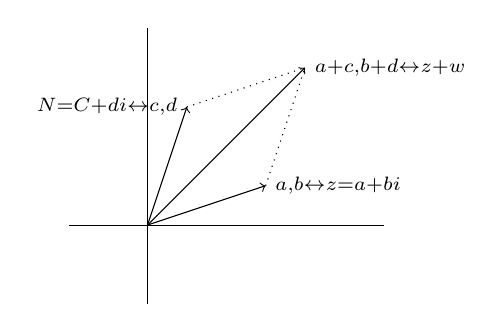
\begin{tikzpicture}
		\draw [-] (-1,0) -- (3,0);
		\draw [-] (0,-1) -- (0,2.5);
		\draw [->] (0,0) -- (0.5,1.5) node[anchor = east]{$\scriptstyle N=C+di\leftrightarrow\lrr{c,d}$};
		\draw [->] (0,0) -- (1.5,0.5) node[anchor = west]{$\scriptstyle \lrr{a,b}\leftrightarrow z=a+bi$};
		\draw [-,dotted] (0.5,1.5) -- (2,2) node[anchor = west]{$\scriptstyle \lrr{a+c,b+d}\leftrightarrow z+w$};
		\draw [-,dotted] (1.5,0.5) -- (2,2);
		\draw [->] (0,0) -- (2,2); 
	\end{tikzpicture}
	%TODO
	\begin{tikzpicture}
		\draw [-] (-2,0) -- (4,0);
		\draw [-] (0,-2) -- (0,4);
		\draw [-] (-.1,1) -- (.1,1) node [anchor=west] {$\scriptstyle i$};
		\draw [-] (1,.1) -- (1,-.1) node [anchor=north] {$\scriptstyle 1$};
		\draw [-] (.1,2) -- (-.1,2) node [anchor=east] {$\scriptstyle b$};
		\draw [-] (2,.1) -- (2,-.1) node [anchor=north] {$\scriptstyle a$};
		\draw (2,2) node [anchor=south west] {$z=a+bi$};
	\end{tikzpicture}

	$Z\rightarrow\overline{Z}$ entspricht Spiegelung an der horizontalen Achse.

	Horizontale Achse: Relle Zahlen\\
	Vertikale Achse: Rein imaginäre Zahlen

	Addition in $\mc$ entspricht der Vektoraddition

	Multiplikation von $a+bi$ mit $c\in\mr$\\
	$c\cdot(a+bi)=ca+cbi$

	\begin{tikzpicture}
	\draw [-] (-1,0) -- (4,0);
	\draw [-] (0,-1) -- (0,4);
	\draw [->] (0,0) -- (3,2) node [anchor=west] {$\scriptstyle (a,b)\leftrightarrow z$};
	\draw [->] (0,0) -- (4.5,3) node [anchor=west] {$\scriptstyle (a,cb)\leftrightarrow c\cdot z$};
	\end{tikzpicture}

	Multiplikation von $a+bi$ mit $i$:\\
	$i\cdot(a+bi)=-b+ai$

	\begin{tikzpicture}
	\draw [-] (-1,0) -- (4,0);
	\draw [-] (0,-1) -- (0,4);
	\draw [-] (0,0) -- (3,1) node [anchor=west] {$(a,b)$};
	\draw [-] (0,0) -- (-1,3) node [anchor=east] {$iz$};
	\draw [-] (3,.1) -- (3,-.1) node [anchor=north] {$a$};
	\draw [-] (-1,.1) -- (-1,-.1) node [anchor=north] {$-b$};
	\draw [-] (.1,1) -- (-.1,1) node [anchor=east] {$b$};
	\draw [-] (.1,2) -- (-.1,2) node [anchor=east] {$a$};
	\end{tikzpicture}

	Entspricht Drehung im $90^\circ$ gegen den Uhrzeigersinn.

	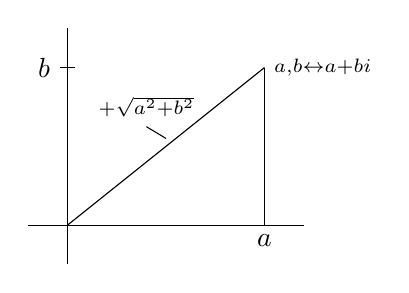
\begin{tikzpicture}
		\draw [-] (-0.5,0) -- (3,0);
		\draw [-] (0,-0.5) -- (0,2.5);
		\draw [-] (2.5,0) node[anchor = north]{$a$} -- (2.5,2) node[anchor = west]{$\scriptstyle \lrr{a,b}\leftrightarrow a+bi$};
		\draw [-] (0,0) -- (2.5,2);
		\draw [-] (1.25,1.1) -- (1,1.25) node[anchor = south]{$\scriptstyle +\sqrt{a^2+b^2}$};
		\draw [-] (.1,2) -- (-.1,2) node [anchor = east]{$b$};
	\end{tikzpicture}

\section{Definition: Absolutbetrag und Abstand}
	\begin{enumerate}[a)]
		\item \textbf{Absolutbetrag} von $z\in\mc$:\\
		$\lrabs{z}=+\sqrt{\mathcal{R}(z)^2+\mathcal{I}(z)^2}\in\mr$\\
		Ist $z\in\mr$, so entspricht das dem üblichen Absolutbetrag in $\mr$.

		Klar:\\
		$\lrabs{\mathcal{R}(z)},\lrabs{I(z)}\leq\lrabs{z}$

		\item Abstand von $z_1,z_2\in\mc$\\
		$d(z_1,z_2):=\lrabs{z_1-z_2}$

		\begin{tikzpicture}
		\draw [-] (-1,0) -- (4,0);
		\draw [-] (0,-1) -- (0,4);
		\draw (1,1) node [anchor=north west] {$\scriptstyle z_2$} -- (3,1) --  (3,2) node [anchor=west] {$\scriptstyle z_1$} -- (1,1);
		\end{tikzpicture}
	\end{enumerate}

\section{Satz: Rechenregeln}
	$z,z_1,z_2\in\mc$
	\begin{enumerate}[a)]
		\item $\overline{(z_1+z_2)}=\overline{z_1}+\overline{z_2}$
		\item $\overline{z_1\cdot z_2}=\overline{z_1}\cdot\overline{z_2}$
		\item $\overline{\overline{z}}=z$
		\item $z=\overline{z}\ \Leftrightarrow\ z\in\mr$
		\item $\lrabs{z}=0\ \Leftrightarrow\ z=0$
		\item $\lrabs{z_1\cdot z_2}=\lrabs{z_1}\cdot\lrabs{z_2}$
		\item $\lrabs{z_1+z_2}\leq\lrabs{z_1}+\lrabs{z_2}$ (Dreiecksregel)
		\item $z\cdot\overline{z}=\lrabs{z}^2$\\
		Für $z\neq 0$ ist $z^{-1}=\frac{1}{\lrabs{z}^2}\cdot\overline{z}$
	\end{enumerate}

\section{Bemerkung: Nullstellen}
	\begin{enumerate}[a)]
		\item In $\mc$ gilt $i^2=-1$\\
			d.h. $x^2+1$ hat eine Nullstelle in $\mc$\\
			(sogar zwei, $i,-i$)\\
			$x^2+1=\lrr{x-1}\lrr{x+i}$

			Es gilt sogar:\\
			$a,b,c\in\mr$, so hat $ax^2+bx+c$ zwei Nullstellen (inklusive Vielfachheit) in $\mc$:\\
			Lösungsformel $x_{1,2}=\dfrac{-b\pm\sqrt{b^2-4ac}}{2a}\quad a\neq 0$\\
			Ist $b^2-4ac\geq 0$, reelle Lösungen.\\
			Ist $b^2-4ac <0$, $\sqrt{b^2-4ac}=\sqrt{-1\lrr{4ac-b^2}}=\sqrt{-1}\cdot \underbrace{\sqrt{4ac-b^2}}_{>0}$\\
			Lösungen in $\mc$:\\
			$x_{1,2} =\dfrac{-b\pm i\sqrt{4ac-b^2}}{2a}$
		\item Sind $a,b,c \in \mc$, so gilt ebenfalls die Lösungsformel.\\
			Man muss also $\sqrt{z}$ bestimmen, $z\in\mc$\\
			$z=u+vi$\\
			Ist $v=0$\\
			$\sqrt{z}=\underbrace{\pm\sqrt{u}}_{u\geq 0}=\underbrace{\pm\sqrt{\lrabs{u}}i}_{u<0}$\\
			Ist $v\neq 0$\\
			$s,t\in\mr$ gesucht mit $\lrr{s+ti}^2=u+vi=\lrr{s^2-t^2}+2sti$\\
			$v=2st\quad u=s^2-t^2$, dabei ist $s,t\neq 0$, da $v\neq 0$\\
			$\Rightarrow$\\
			$s=\frac{v}{2t}\quad\frac{v^2}{4t^2}-t^2=u$\\
			$v^2-4t^4=4ut^2$, setze $d=t^2$\\
			$4d^2+4ud-v^2=0$\\
			$d=\dfrac{-u+\sqrt{u^2+v^2}}{2}$, $+$-Zeichen vor der Wurzel, da $d\geq 0$\\
			$t=\pm\sqrt{\dfrac{-u+\sqrt{u^2+v^2}}{2}}$
	\end{enumerate}

\section{Fundamentalsatz der Algebra}
	C.F.Gauß, 1777-1855

	Jedes Polynom $f\in\mc\lra{x}$ vom Grad $n\geq 1$ hat (einschließlich Vielfachhalt) genau $n$ Nullstellen in $\mc$, das heißt es existiert $b_1,\dots,b_n\in\mc$ (nicht notwendig verschieden), so dass $f=a_n\lrr{x-b_1}\lrr{x-b_2}\dots\lrr{x-b_n}$, dabei ist $a_n$ der höchste Koeffizient von $f$. \\
	Insbesondere: In $\mc\lra{x}$ haben irreduzible Polynome $\grad\lrr{1}$

\section{Korollar: irreduzible Polynome}
	Irreduzible Polynome in $\mr\lra{x}$ haben $\grad\leq 2$. Ist $f$ irreduzibel vom $\grad\ 2$, normiert, so \\
	$f=\lrr{x-z}\lrr{x-\overline{z}}$ für ein $z\in\mc\mnot\mr$

	\textbf{Beweis}

	Sei $f\in\mr\lra{x}$ irreduzibel, normiert, $\grad\lrr{f}=2$\\
	Nach 2.8 hat $f$ Nullstelle $z\in\mc\mnot\mr$\\
	$f(x)=x^2+bx+c\quad b,c\in\mr$\\
	$0=f(z)=z^2+bz+c$\\
	$0=\overline{0}=\overline{z^2+bz+c} \underset{\mbox{\scriptsize 2.6}}{=}\overline{z}^2+\overline{b}\cdot\overline{z}+\overline{c}=\overline{z}^2+b\cdot\overline{z}+c$, da $b,c\in\mr$\\
	$f\lrr{\overline{z}}=0$\\
	$z\neq\overline{z}$, nach 1.36: $\lrr{x-z}\lrr{x-\overline{z}}$ teilt $f$ in $\mc\lra{x}$\\
	In $\mc\lra{x}$:\\
	$f=g\cdot\lrr{x-z}\lrr{x-\overline{z}}$ für ein $g\in\mc\lra{x}$\\
	$\underbrace{\lrr{x-z}\lrr{x-\overline{z}}}_{\in\mr\lra{x}}=x^2-\underbrace{\lrr{z+\overline{z}}}_{\in\mr}x+\underbrace{z\overline{z}}_{\scriptstyle \lrabs{z}^2\in\mr}$\\
	$f\in\mr\lra{x}\Rightarrow g\in\mr\lra{x}$\\
	$f$ ist irreduzibel in $\mr\lra{x}$ normiert $\Rightarrow g=1$\\
	$f\lrr{x}=\lrr{x-z}\lrr{x-\overline{z}}$

\section{Bemerkung: Absolutbetrag, Multiplikation und Wurzel}
	\begin{enumerate}[a)]
		\item Alle komplexen Zahlen von gleichem Absolutbetrag $r$ liegen auf Kreislinie vom Radius $r$ um $(0,0)$

			\begin{tikzpicture}
				\draw (0,0) circle (2);
				\draw [] (0,0) -- node [anchor=south] {$r$} (1.41,1.41) node [anchor=south west] {$z,\ r=\lrabs{z}$} -- (1.41,0);
				\draw (7mm,0mm) arc (0:45:7mm);
				\draw (.1,-.2) node [anchor=south west] {$\varphi$};
				\draw [dashed] (-3,0) -- (3,0);
				\draw [dashed] (0,-3) -- (0,3);
				\draw [<-] (1.41,0.7) -- (2.5,0.7) node [anchor=west] {$\lrabs{z}\cdot\sin(\varphi)$};
				\draw [<-] (0.8,0) -- (0.8,-.5) node [fill=white,anchor=north] {$a=b$};
			\end{tikzpicture}

			$z=\lrabs{z}\cdot\cos\lrr{\varphi}+i\lrabs{z}\cdot\sin\lrr{\varphi}$\\
			$z=\lrabs{z}\lrr{\cos\lrr{\varphi}+i\sin\lrr{\varphi}}=r\cdot\lrr{\cos\lrr{\varphi}+i\sin\lrr{\varphi}}$

			Diese Darstellung entspricht den \textbf{Polarkoordinaten} $\lrr{r,\varphi}$ von einem Punkt im $\mr^2$, der der zahl $z$ entspricht.
		\item \begin{align*}
				z_1\cdot z_2=&\lrabs{z_1}\cdot\lrr{\cos\lrr{\varphi_1}+i\sin\lrr{\varphi_1}}\cdot\lrabs{z_2}\cdot\lrr{\cos\lrr{\varphi_2}+i\sin\lrr{\varphi_2}}\\
				=&\lrabs{z_1}\lrabs{z_2}(\cos\lrr{\varphi_1}\cos\lrr{\varphi_2}-\sin\lrr{\varphi_1}\sin\lrr{\varphi_2}\\
				&+\lrr{\cos\lrr{\varphi_1}\sin\lrr{\varphi_2}+\sin\lrr{\varphi_1}\cos\varphi_2}i)\\
				z_1\cdot z_2=&\lrabs{z_1}\cdot\lrabs{z_2}\lrr{\cos\lrr{\varphi_1+\varphi_2}+i\sin\lrr{\varphi_1+\varphi2}}
			\end{align*}
			(letzter Schritt verwendet das Additionstheorem der Trigonometrie)

			Führt zu Veranschaulichung der Multiplikation:

			\begin{tikzpicture}
				\draw [dashed] (-3,0) -- (3,0);
				\draw [dashed] (0,-3) -- (0,3);
				\draw [->] (0,0) -- node [anchor=south] {$\scriptstyle\lrabs{z_1}$} (2,0.5) node [anchor=west] {$z_1$};
				\draw [->] (0,0) -- node [anchor=east] {$\scriptstyle\lrabs{z_2}$} (1,2) node [anchor=south west] {$z_2$};
				\draw (7mm,0mm) arc (0:14.03:7mm);
				\draw (5mm,0mm) arc (0:63.43:5mm);
				\draw [red] (9mm,0mm) arc (0:77.46:9mm);
				\draw [->,red] (0,0) -- node [anchor=east] {$\scriptstyle z_1\cdot z_2$} (0.9,4) node [anchor=west] {{\scriptsize Länge} $\scriptstyle \lrabs{z_1}\cdot\lrabs{z_2}$};
				\draw [<-,red] (0.64,0.64) -- (1.2,1.2) node [anchor=west] {$\scriptstyle \varphi_1 + \varphi_2$};
			\end{tikzpicture}

			Insbesondere:\\
			$z=\lrabs{z}\cdot\lrr{\cos\lrr{\varphi}+i\sin\lrr{\varphi}}$\\
			$z^2=\lrabs{z}^2\lrr{\cos\lrr{2\varphi}+i\sin\lrr{2\varphi}}$
		\item Wurzelberechnung einer komplexen Zahl\\
			geg. $w\in\mc$, ges. ist $z\in\mc$ mit $z^2=2\Leftrightarrow z=\sqrt{w}$\\
			$w=\lrabs{w}\cdot\lrr{\cos\lrr{\varphi}+i\sin\lrr{\varphi}}$\\
			$z=\pm\sqrt{\lrabs{w}}\lrr{\cos\lrr{\frac{4}{2}}+i\sin\lrr{\frac{4}{2}}}$

			Grenzbegriff für reelle Folgen\\
			$\lrr{a_n}\rightarrow c\in\mr$\\
			$\forall\epsilon >0\exists n_0\lrr{\epsilon}\forall n\geq n_0\lrr{\epsilon}:\lrabs{a_n-c}<\epsilon$\\
			Mit Absolutbetrag in $\mc$ lässt sich diese Definition auf Konvergenz von komplexen Zahlenfolgen wörtlich übertragen.\\
			Insbesondere lässt sich die Konvergenz von Reihen in $\mc$ definieren als\\
			$\limsum{i=0}{\infty}a_i\quad\lrr{\mbox{Konvergenz } \lrr{s_n} \mbox{ mit } s_n=\limsum{i=0}{n}a_i}$

			Wie in $\mr$ folgt auch in $\mc$ aus der absoluten konvergenz einer Reihe die normale Konvergenz:\\
			$a_i\in\mc$\\
			$\limsum{i=0}{\infty}\lrabs{a_i}$ konvergiert $\Rightarrow \limsum{i=0}{\infty}a_i$ konvergiert.
	\end{enumerate}

\section{Definition: Komplexe Exponentialfunktion}
	Für jedes $z\in\mc$ konvergiert $\limsum{k=0}{\infty}\frac{z^k}{k!}=:\exp\lrr{z}$\\
	\textbf{komplexe Exponentialfunktion}\\
	Schreibweise:\\
	$e^z$ statt $\exp\lrr{z}$

\section{Satz: Euler'sche Formel}
	\begin{enumerate}[a)]
		\item $e^{z_1}\cdot e^{z_2}=e^{z_1+z_2}$ für alle $z_1,z_2\in\mc$
		\item $e^{it}=\cos\lrr{t}+i\cdot\sin\lrr{t}$ für alle $t\in\mr$\\
			(Euler'sche Formel)\\
			$\lrabs{e^{it}}=1$\\
			$e^{it}=e^{i\lrr{t+2k\pi}}$\\
			$e^{-it}=\overline{e^{it}}$

			\begin{tikzpicture}
				\draw [dashed] (-2,0) -- (2,0);
				\draw [dashed] (0,-2) -- (0,2);
				\draw [] (0,0) circle (1);
				\draw [] (-1,.1) -- (-1,-.1) node [anchor=north east] {$\scriptstyle -1$};
				\draw [] (1,.1) -- (1,-.1) node [anchor=north west] {$\scriptstyle 1$};
				\draw [] (-.1,-1) -- (.1,-1) node [anchor=north west] {$\scriptstyle -i$};
				\draw [] (-.1,1) -- (.1,1) node [anchor=south west] {$\scriptstyle i$};
				\draw (7mm,0mm) arc (0:30:7mm);
				\draw [] (.5,.15) node [] {$\scriptstyle t$};
				\draw [] (0,0) -- (0.85,0.55) node [anchor=south west] {$e^{it}$};
			\end{tikzpicture}
		\item $\lrabs{e^z}=e^{\Re\lrr{z}}$
		\item $e^z=e^{\Re(z)}\lrr{\cos\lrr{\Im(z)}+i\sin\lrr{\Im(z)}}$\\
			$\lra{e^{2+5i}=e^2\lrr{\cos\lrr{5}+i\sin\lrr{5}}}$
		\item Jede komplexe Zahl $z$ lässt sich in der Form $z=r\cdot e^{i\varphi}$ mit $r\in\mr\quad r\geq 0$ und $\varphi\in\mr$, $0\leq\varphi <2\pi$. Ist $r\neq 0$, so ist die Darstellung eindeutig (\textbf{Polarform})\\
			$\lrr{r,\varphi}$ Polarkoordinaten von $z$
	\end{enumerate}
	\textbf{Beweis}
	\begin{enumerate}[a)]
		\item Wie in $\mr$
		\item 
			\begin{align*}
				e^{it}&=\suminf{k=0}\frac{\lrr{it}^k}{k!}\\
				&=\suminf{j=0}\frac{\lrr{it}^{2j}}{\lrr{2j}!}+\suminf{j=0}\frac{\lrr{it}^{2j+1}}{\lrr{2j+1}!}\\
				&=\underbrace{\suminf{j=0}\lrr{-1}^j\frac{t^{2j}}{\lrr{2j}!}}_{\cos\lrr{t}}+i\underbrace{\suminf{j=0}\lrr{-1}^j\frac{t^{2j+1}}{\lrr{2j+1}!}}_{\sin\lrr{t}}
			\end{align*}
			(Das nennt sich später Taylor-Reihe)
			\begin{align*}
				e^{-it}&=\cos\lrr{-t}+i\sin\lrr{-t}\\
				&=\cos\lrr{t}-i\sin\lrr{t}\\
				&=\overline{e^{it}}\\
				\lrabs{e^{it}}&=+\sqrt{\cos^2\lrr{t}+\sin^2\lrr{t}}=1
			\end{align*}
		\item d) nachrechnen
		\item folgt aus b) und 2.10a)
	\end{enumerate}

\section{Bemerkung}
	$z_j=r_j\cdot e^{i\varphi_j}\quad j=1,2$\\
	$z_1\cdot z_2=\underline{r_1\cdot r_2}\cdot e^{i\lrr{\varphi_1+\varphi_2}}$ (2.12a))\\
	(vgl. 2.10b))

\section{Bemerkung}
	$\mc$ hat gute algebraische und analytische Eigenschaften (noch bessere als $\mr$).\\
	\textbf{Aber}: Es gibt \textbf{keine} totale Ordnung $\leq$ auf $\mc$ mit folgenden Eigenschaften:
	\begin{itemize}
		\item $a\leq b, c\leq d \quad \Rightarrow \quad a+c\leq b+d$
		\item $a\leq b, r\geq 0 \quad \Rightarrow \quad ar\leq br$\\
			(das gilt in $\mr$ bezüglich der normalen $\leq$-Relation)
	\end{itemize}
